\documentclass{article}
\usepackage[section]{placeins}
\usepackage{graphicx}
\usepackage{wrapfig}

\usepackage{hyperref}
\hypersetup{
    colorlinks=true,
    linkcolor=blue,
    filecolor=magenta,      
    urlcolor=cyan,
    pdftitle={Overleaf Example},
    pdfpagemode=FullScreen,
    }

\author{Yaghoub Shahmari}
\title{Report - Problem Set No 4}
\date{\today}
\graphicspath{ {../Figs/} }

\begin{document}
    \maketitle
    \section*{Problem 1}
    \textbf{Basic description:}
    In this problem, we try to find the chance of being connected to the infinite cluster again.
    The difference from the previous attempt is that I use the fraction of the size of the infinite
    cluster to the size of the whole network. So all of the previous steps will go through.

    \textbf{Results:}

    \begin{figure}[!htb]
        \centering
        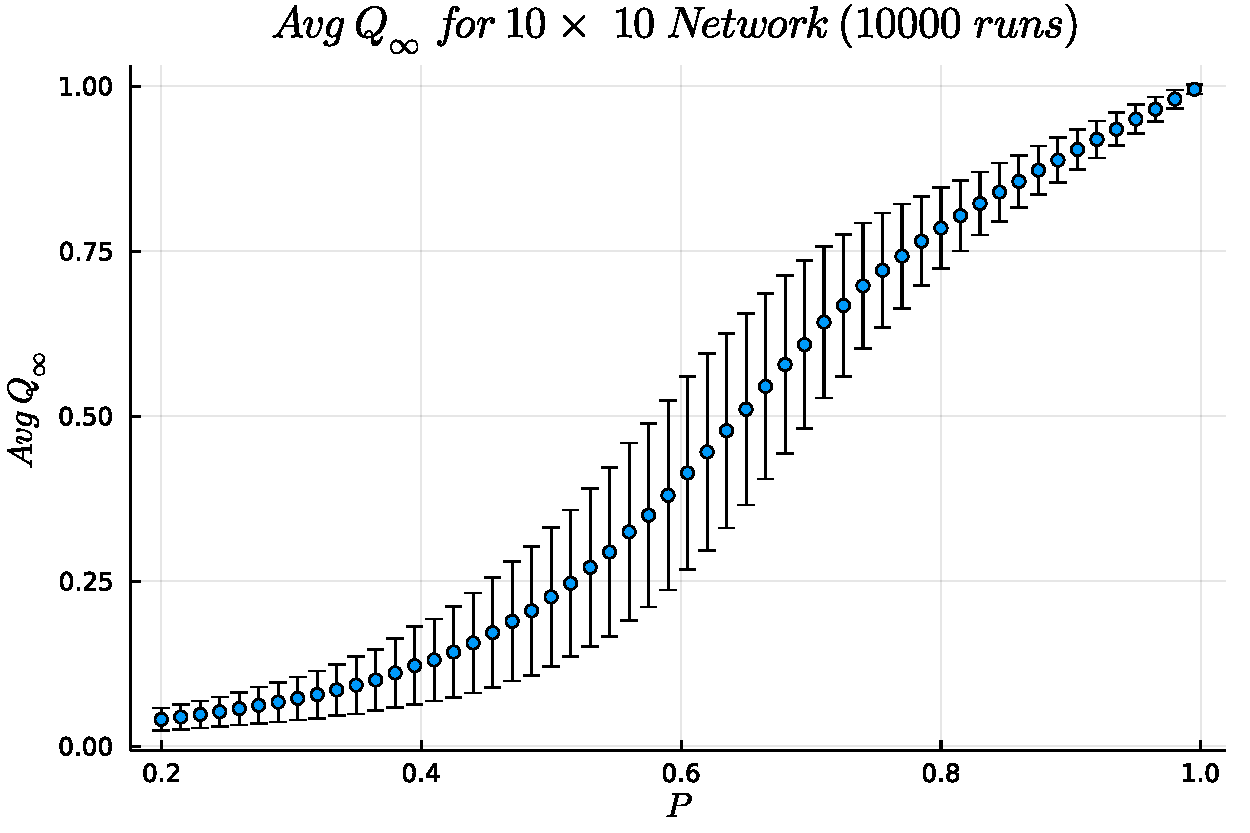
\includegraphics[scale = 0.275]{/Q1/dim10-10000}
        \label{fig:1.1}
        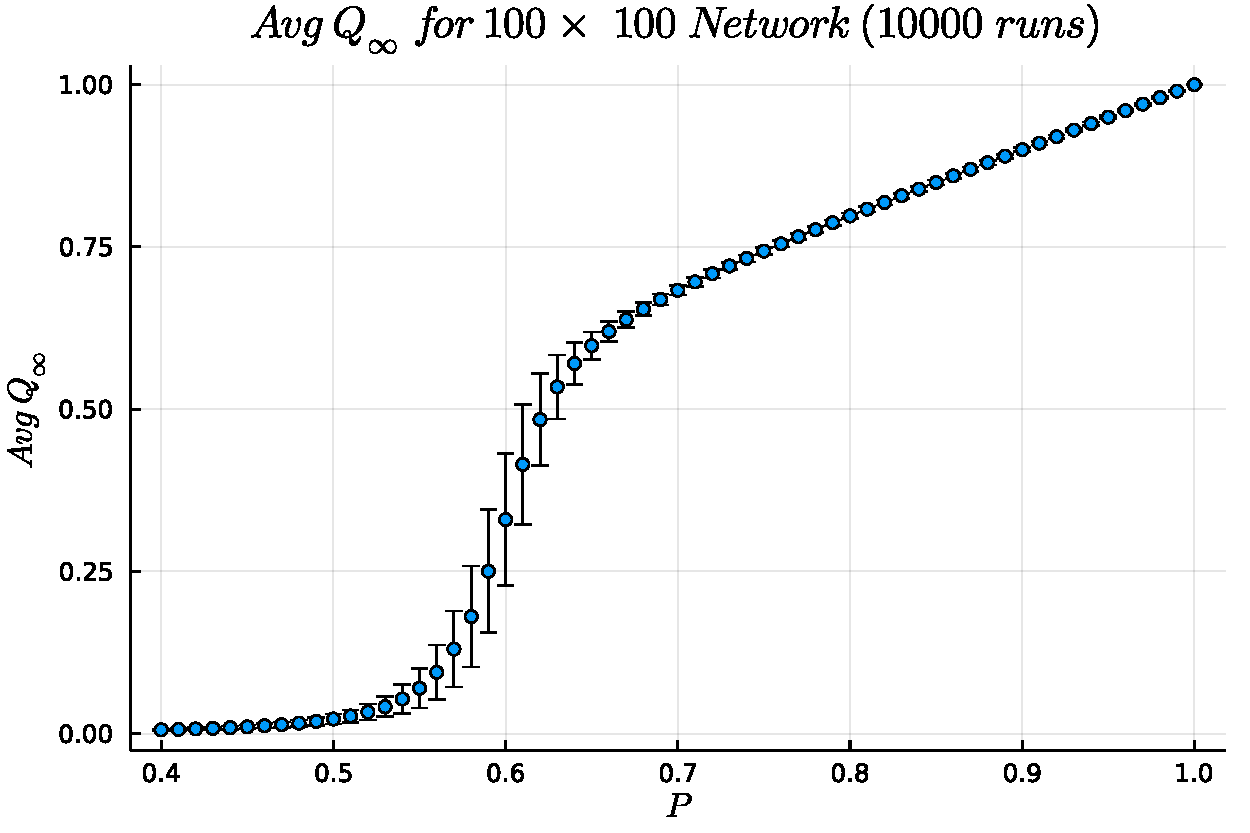
\includegraphics[scale = 0.275]{/Q1/dim100-10000}
        \label{fig:1.2}
        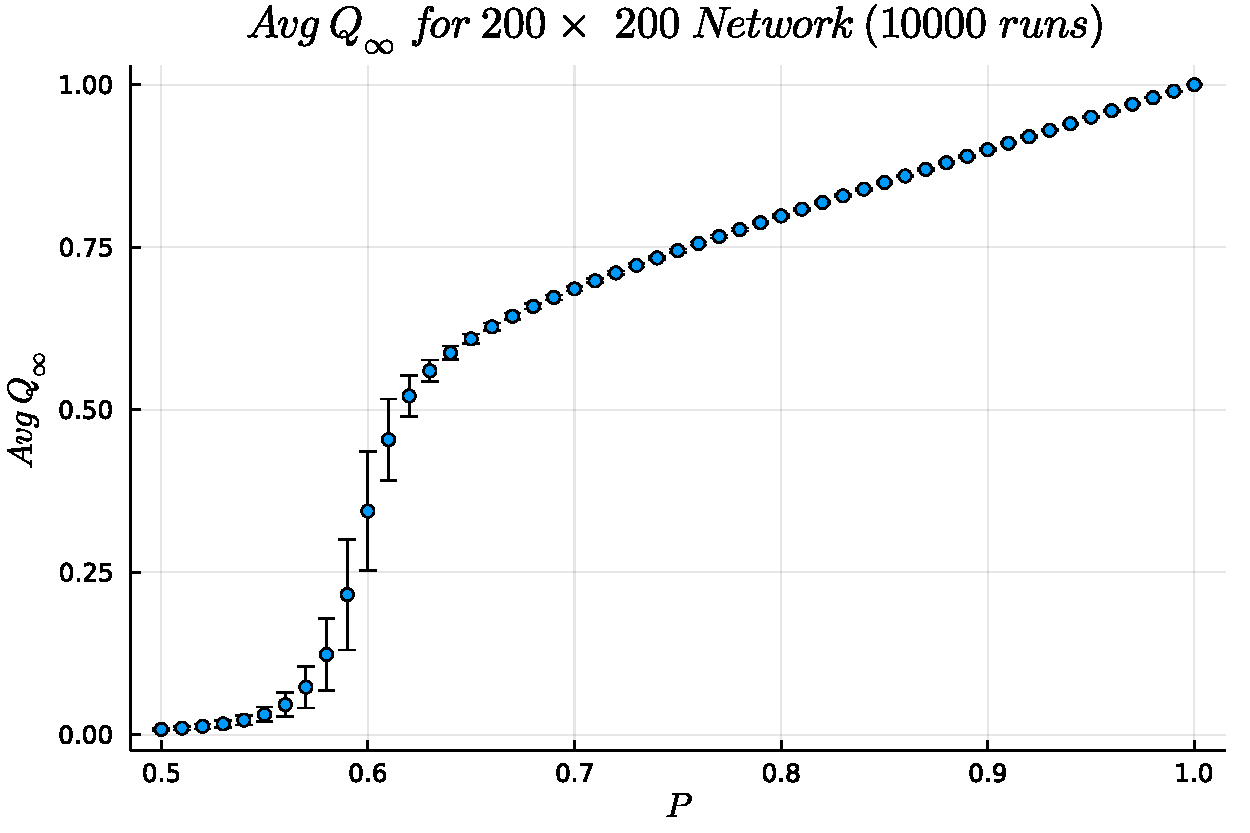
\includegraphics[scale = 0.4]{/Q1/dim200-10000}
        \label{fig:1.3}
        \caption{$Q_{\infty}$ for $L=10, 100, 200$}
    \end{figure}

    \pagebreak

    \section*{Problem 2}
    \textbf{Basic description:}

    In this problem, we try to find the correlation length of percolation of grid graphs.
    In this case, we will find the largest finite cluster.
    Then, we have to calculate the gyration radius of that cluster as the book told us.
    and finally, we will run the calculation and average the data.

    \textbf{Results:}

    \begin{figure}[!htb]
        \centering
        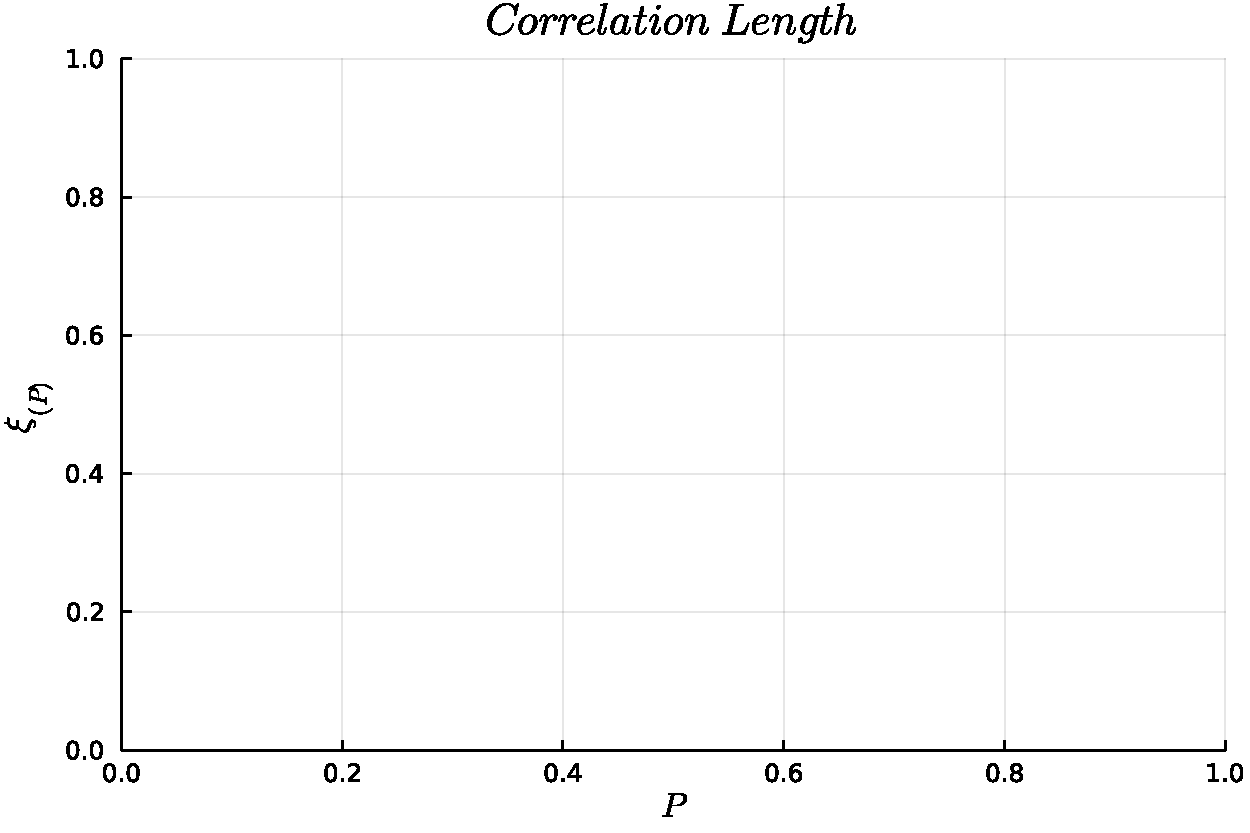
\includegraphics[scale = 0.2]{/Q2/CL}
        \label{fig:2.1}
        \caption{$Q_{\infty}$ for $L=10, 100, 200$}
    \end{figure}

    \textbf{Extrapolation results:}

    To find the requested parameters ($\nu$ and $Pc_{\infty}$),
    we have to do previous steps for several $P$ and $L$.
    After exporting data, we use the Curvefit function in the LsqFit library.
    Given that we intend to find the parameters and improve the
    accuracy we will consider that we know one of the parameters (find the amount from the internet)
    and find the other using the mentioned method.

    \begin{figure}[!htb]
        \centering
        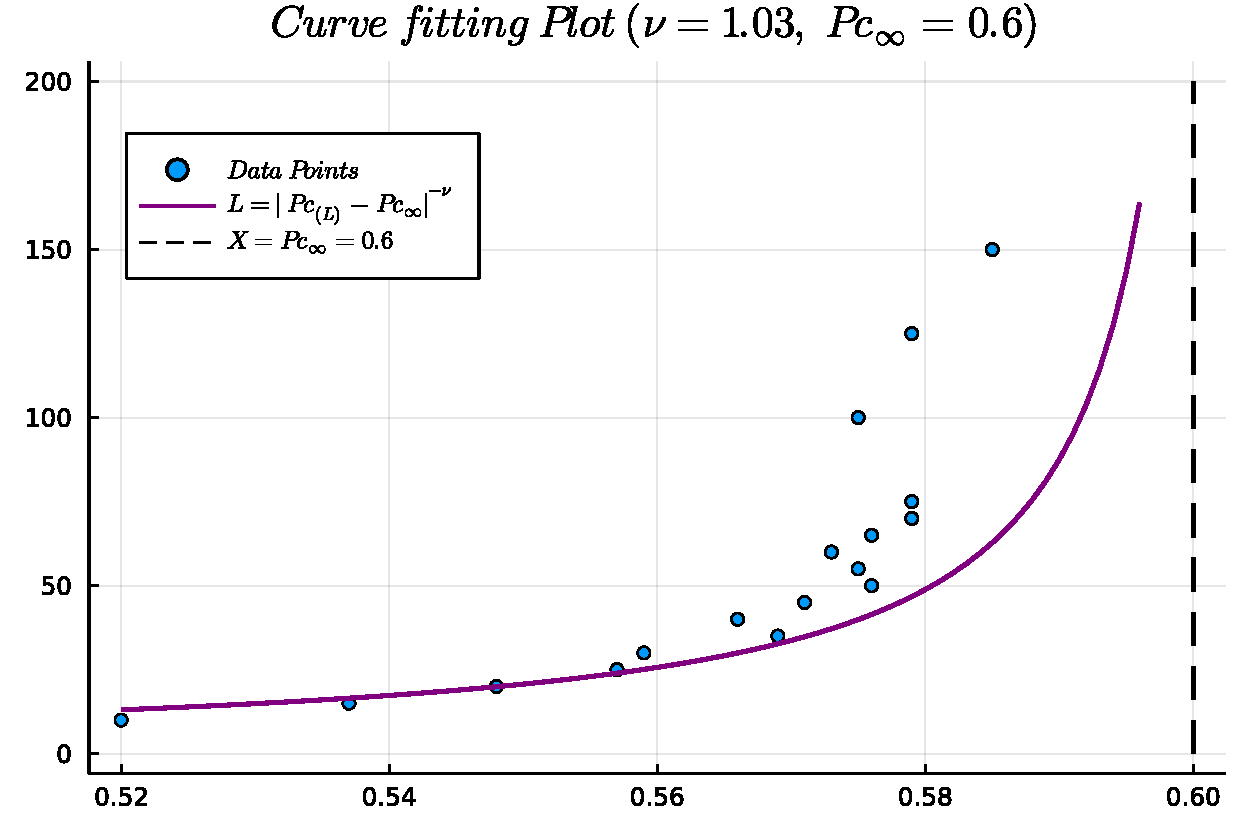
\includegraphics[scale = 0.35]{/Q2/Q2-CF-res}
        \label{fig:2.2}
        \caption{Curvefit result for exported data}
    \end{figure}
    
    \section*{Problem 3}
    \textbf{Basic description:}

    In this problem, we want to find the cluster fractal dimension in the grid network percolation.
    In this case, we deploy the cluster grow algorithm,
    find the size and gyration radius of the created cluster,
    and export the data of ensemble we need for all parts.

    \textbf{Results:}

    \begin{figure}[!htb]
        \centering
        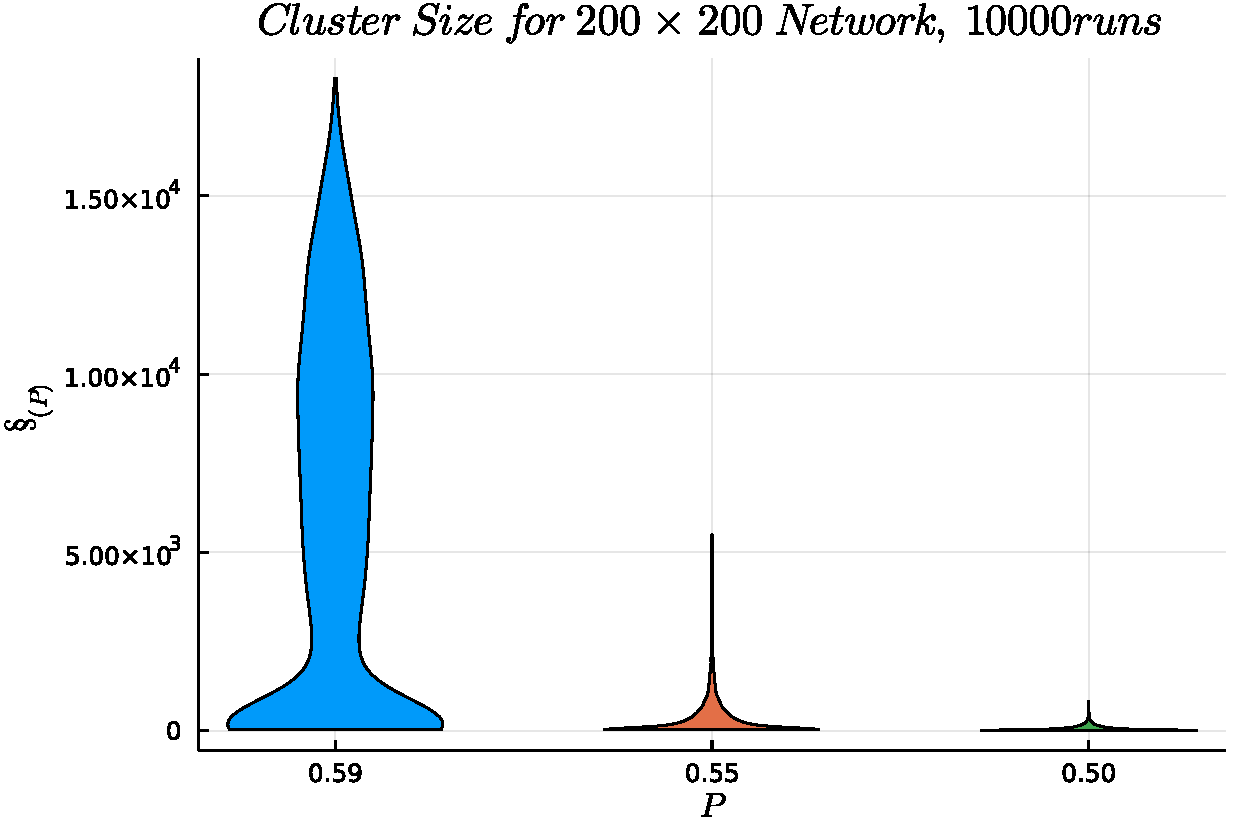
\includegraphics[scale = 0.25]{/Q3/Q3-S-violon}
        \label{fig:3.1}
        \includegraphics[scale = 0.25]{/Q3/Q3-XI-violon}
        \label{fig:3.2}
        \includegraphics[scale = 0.25]{/Q3/Q3-XI-hist}
        \label{fig:3.3}
        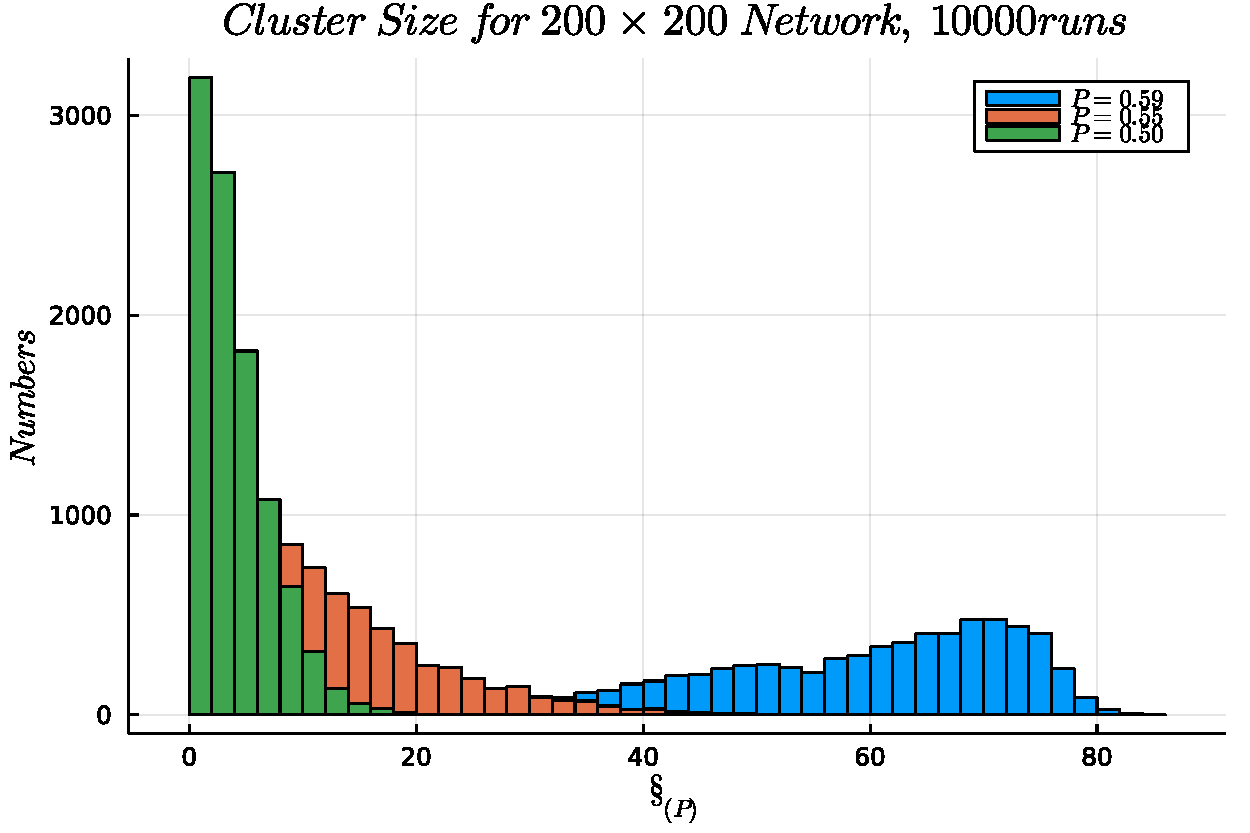
\includegraphics[scale = 0.25]{/Q3/Q3-S-hist}
        \label{fig:3.4}
        \caption{Figures of ensemble of wanted P data}
    \end{figure}
        
    \begin{figure}[!htb]
        \centering
        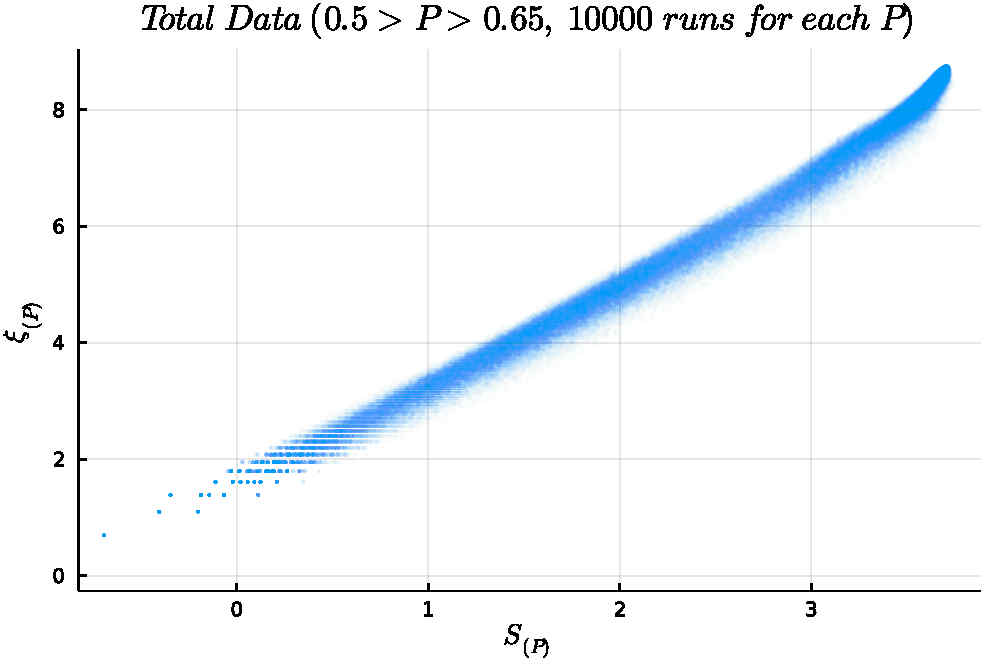
\includegraphics[scale = 0.25]{/Q3/Q3-S-XI.jpg}
        \label{fig:3.5}
        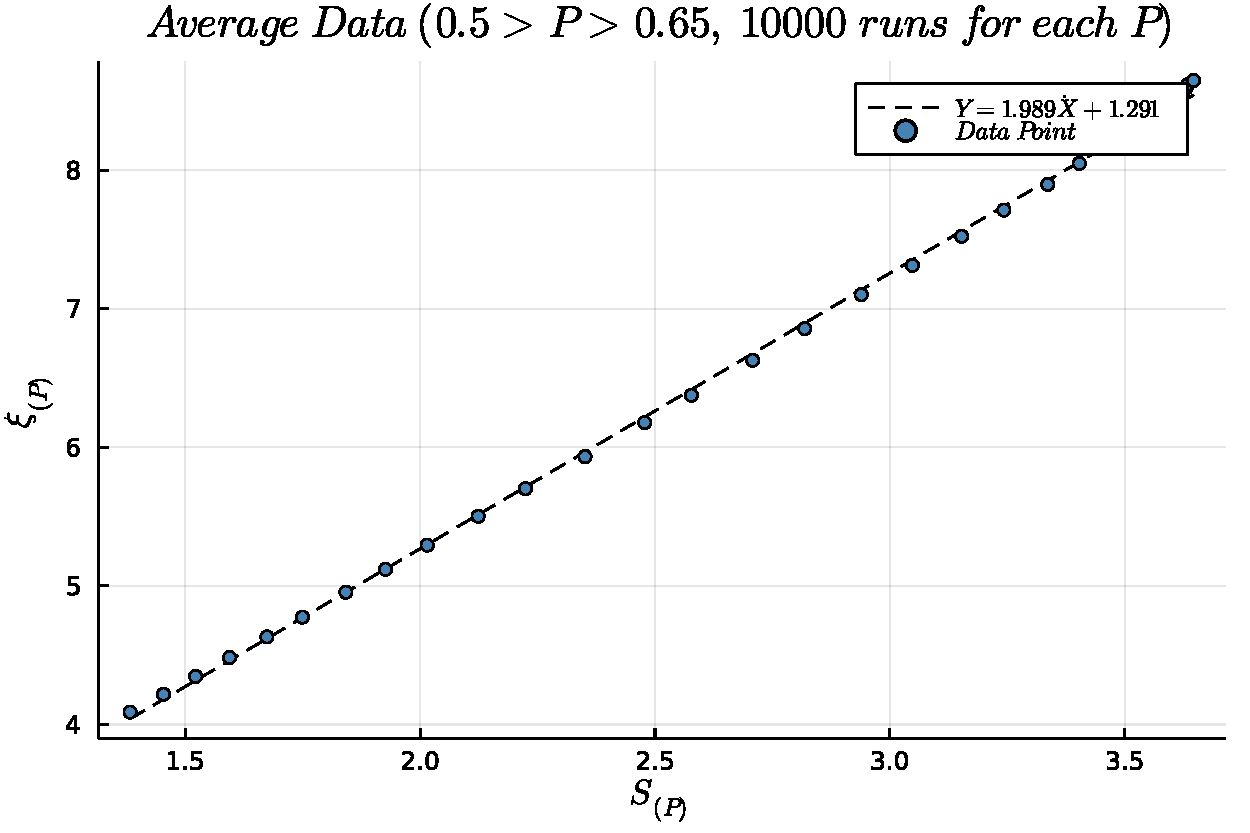
\includegraphics[scale = 0.25]{/Q3/Q3-S-XI-Avg}
        \label{fig:3.6}
        \caption{Scatter and average of total data. The line slope is equal to the cluster fractal dimension.
        The axis is log scaled.}
    \end{figure}

    There is also a few animation in the Figs flolder for cluster grows.

    \section*{Problem 4}
    \textbf{Basic description:}

    In this problem, we want to simulate the 1D Random Walk.
    The Random Walker coded as the book explained it.
    The plots show the simulation for the 10000 time-steps for different P and $X_0 = 0$.
    
    \textbf{Results:}

    \begin{figure}[!htb]
        \centering
        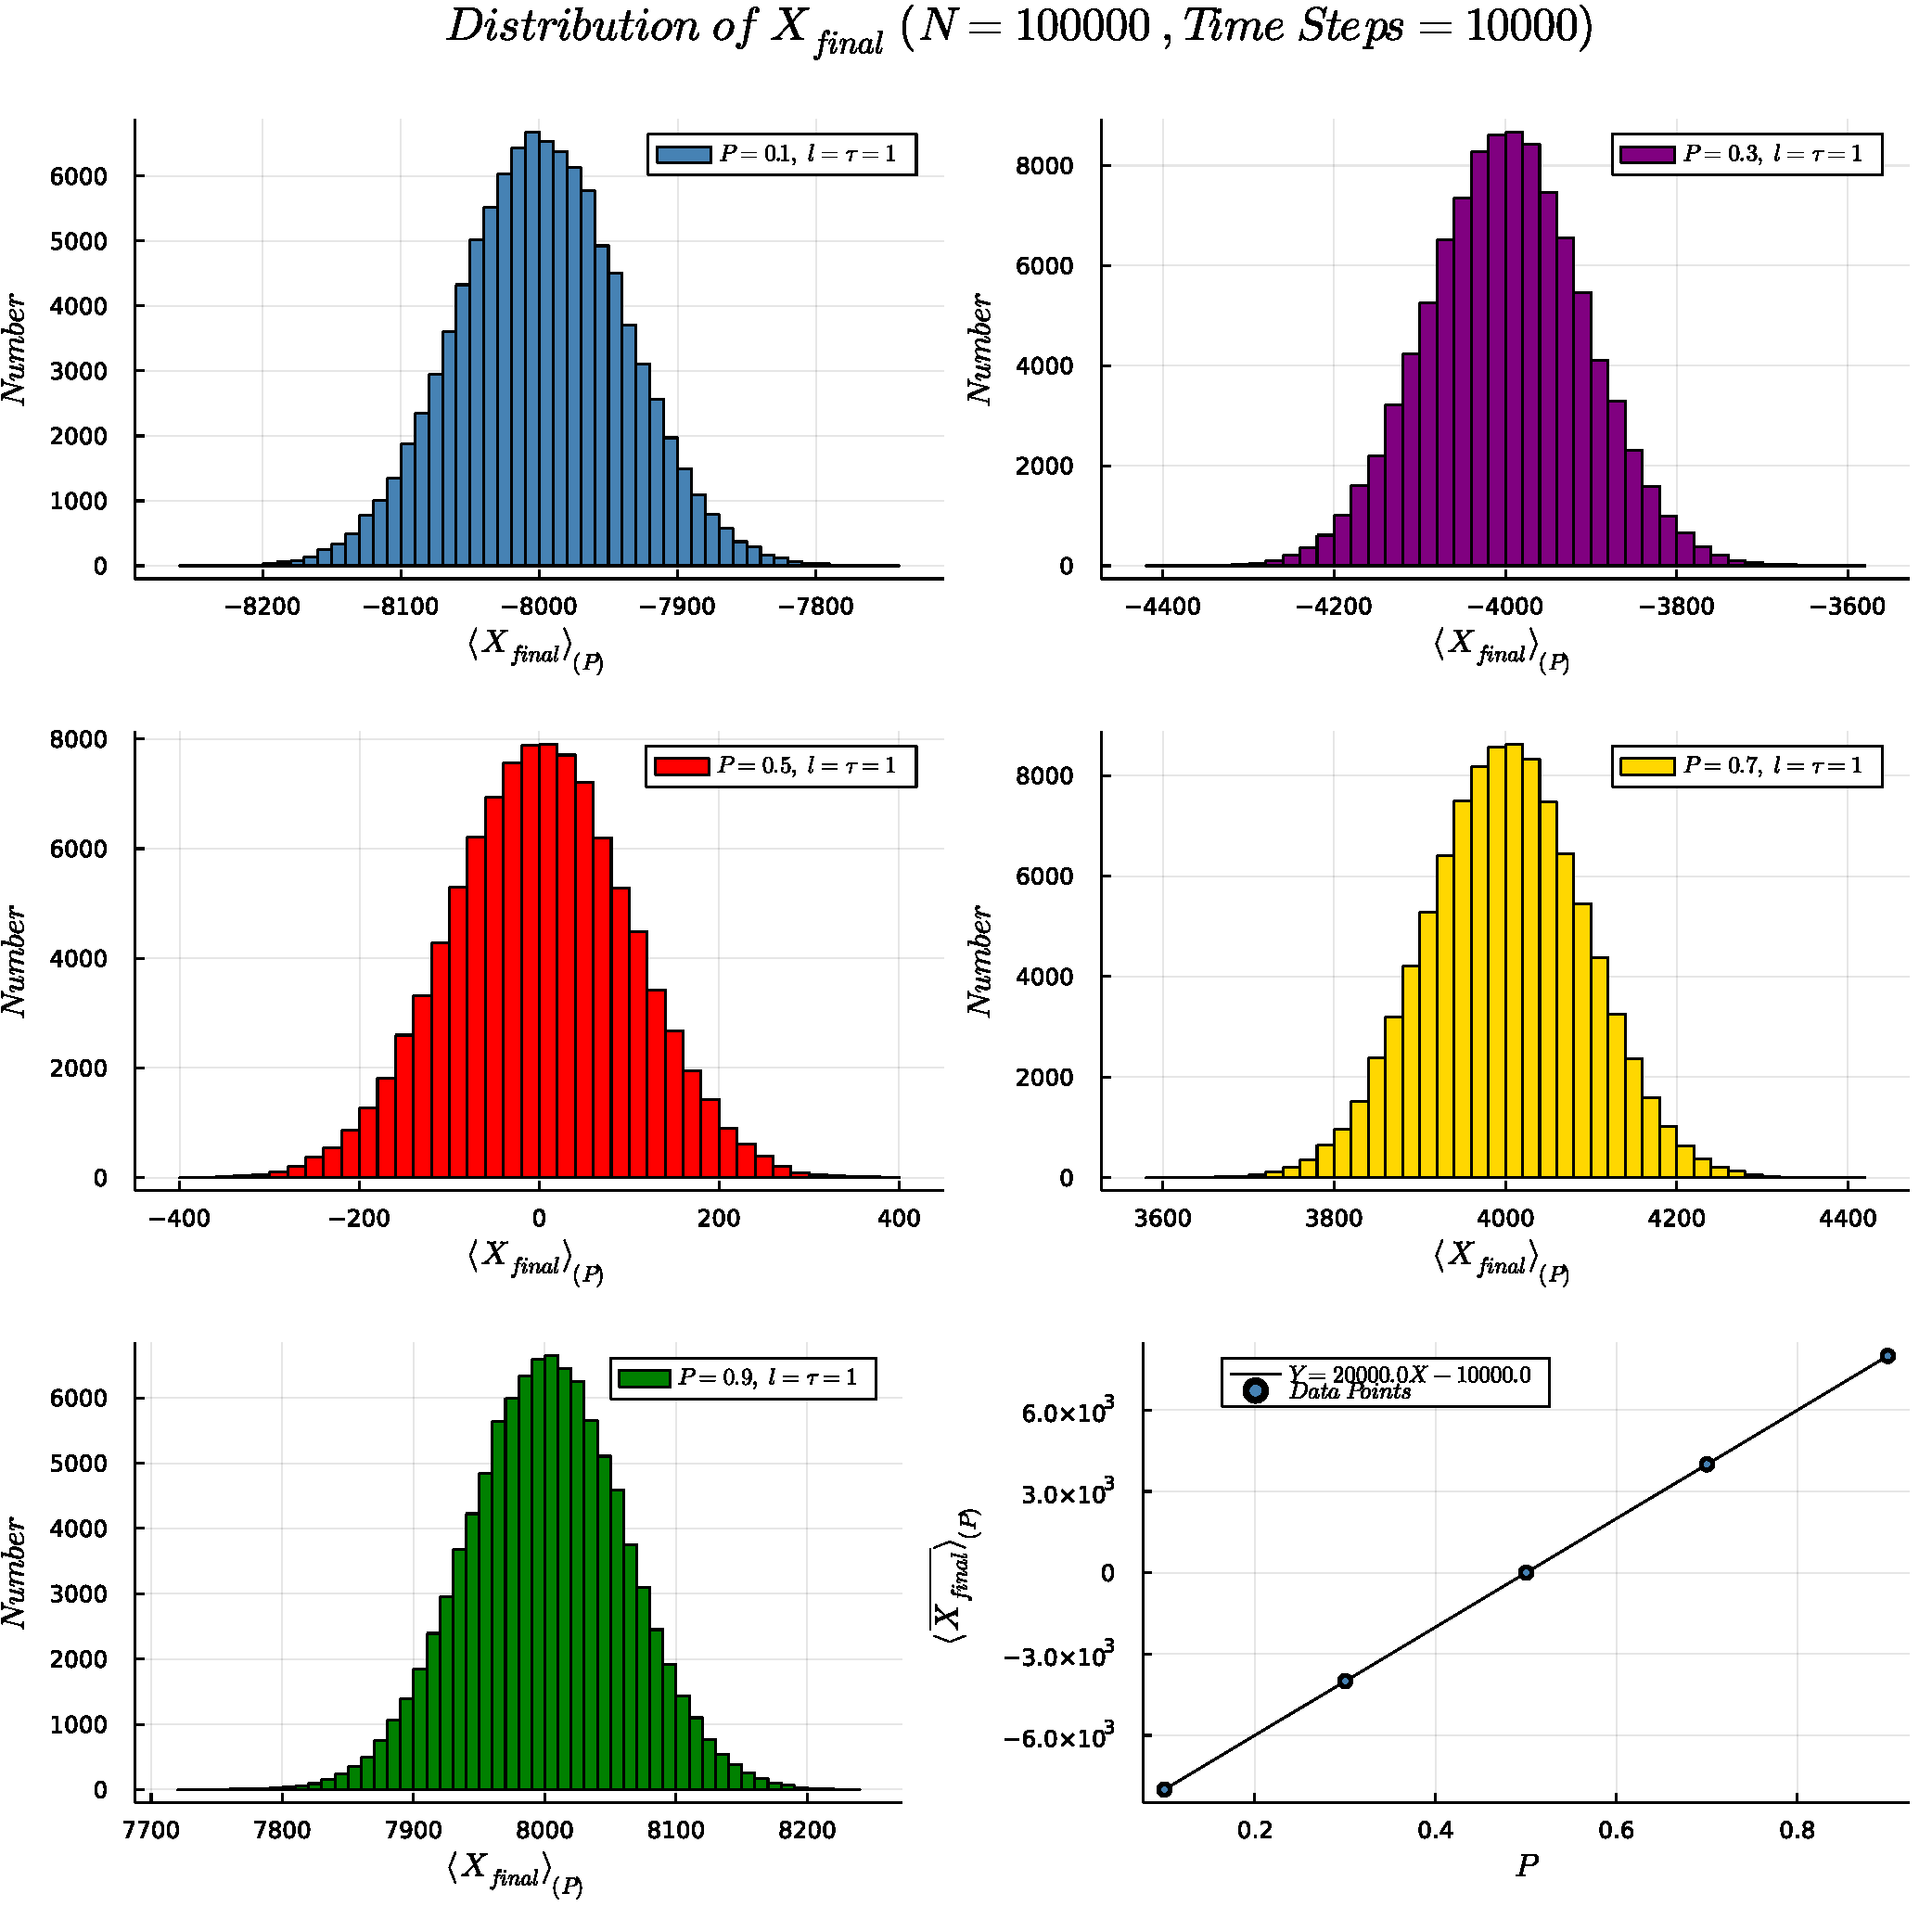
\includegraphics[scale = 0.3]{/Q4/Q4-tot}
        \label{fig:4.1}
        \caption{The histogram plots for exported data and average $X_{final}$ for each.}
    \end{figure}

    \pagebreak

    \section*{Problem 5}
    \textbf{Basic description:}

    In this problem, we add a condition to the previous simulation.
    We consider that twenty surface steps are surrounded by traps and in every step,
    we check if the random walker is trapped or not.
    After being trapped, we return the time steps that the Random walker was walking.
    ($\tau\ \& \ l = 1$).

    \textbf{Results:}

    \begin{figure}[!htb]
        \centering
        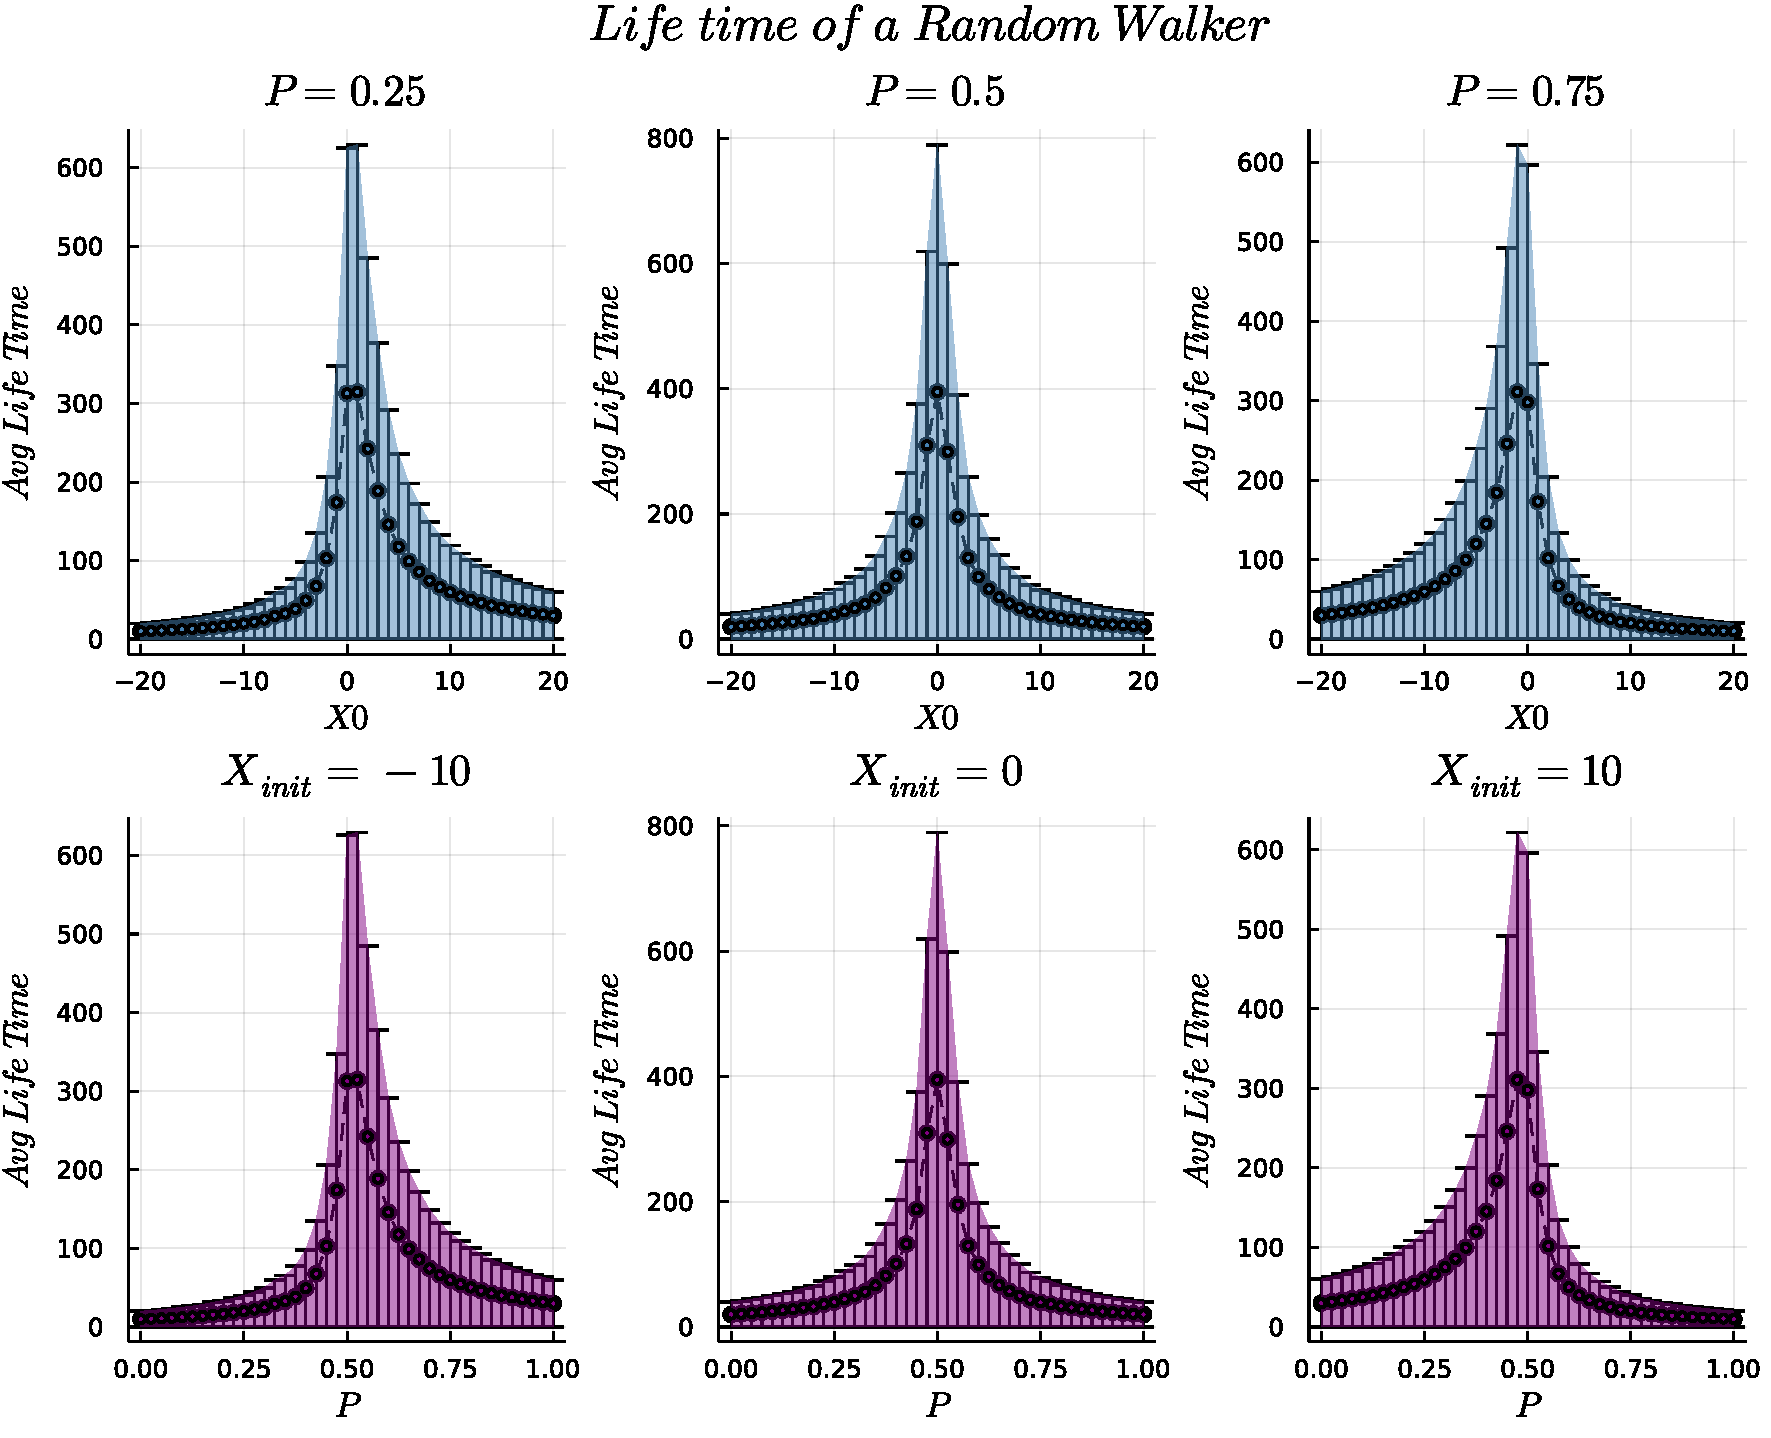
\includegraphics[scale = 0.25]{/Q5/Q5-scat}
        \label{fig:5.1}
        \caption{The Scatter figures for several $X_0$ and $P$ and average $X_{final}$ for each.}
    \end{figure}

    \begin{figure}[!htb]
        \centering
        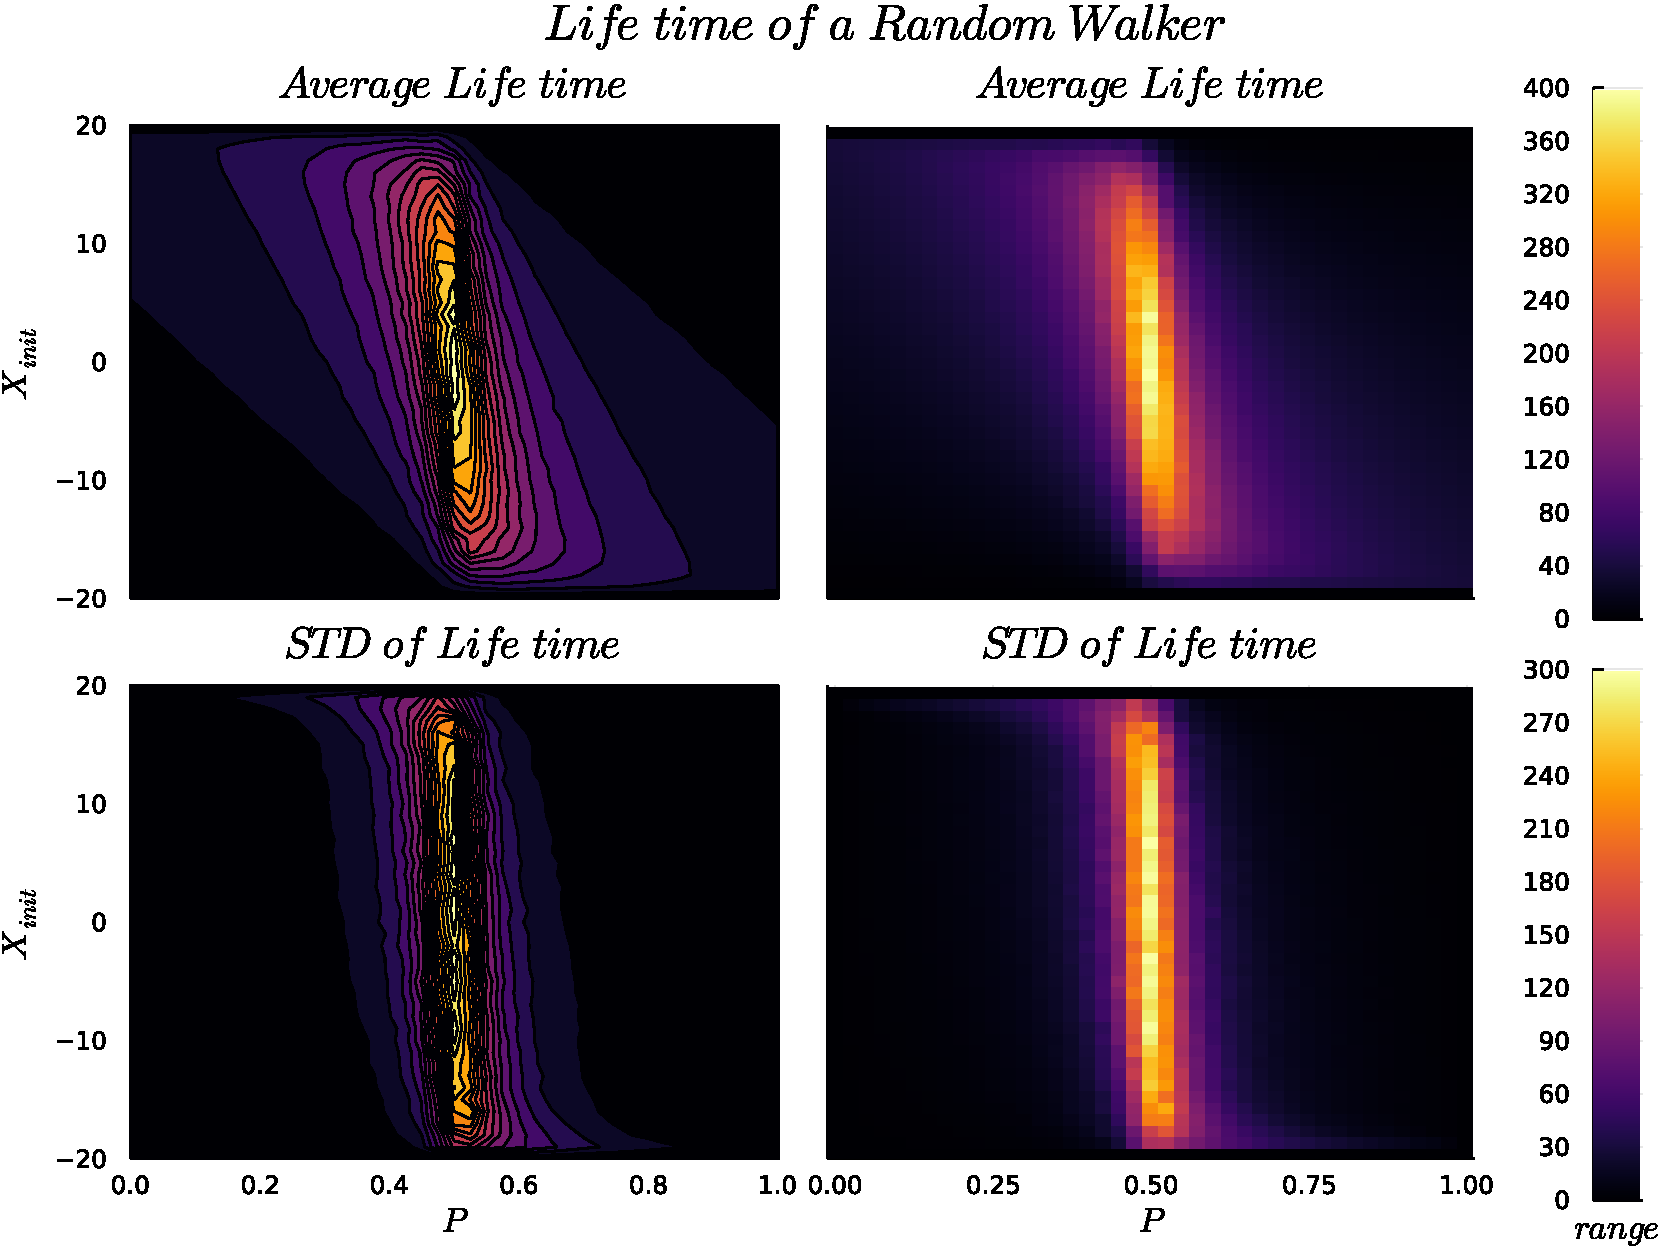
\includegraphics[scale = 0.3]{/Q5/Q5-cont}
        \label{fig:5.2}
        \caption{The contour figures for all possible $X_0$ and $P$ and average and STD $X_{final}$ for each state.}
    \end{figure}

    \section*{Problem 6}
    \textbf{Basic description:}

    In this problem, we code a deterministic algorithm
    that calculates the presence density of a random walker
    on a cell on each time step for a trapped situation.
    Then we find when the random walker presence density will be near to 1.

    \textbf{Results:}

    \begin{figure}[!htb]
        \centering
        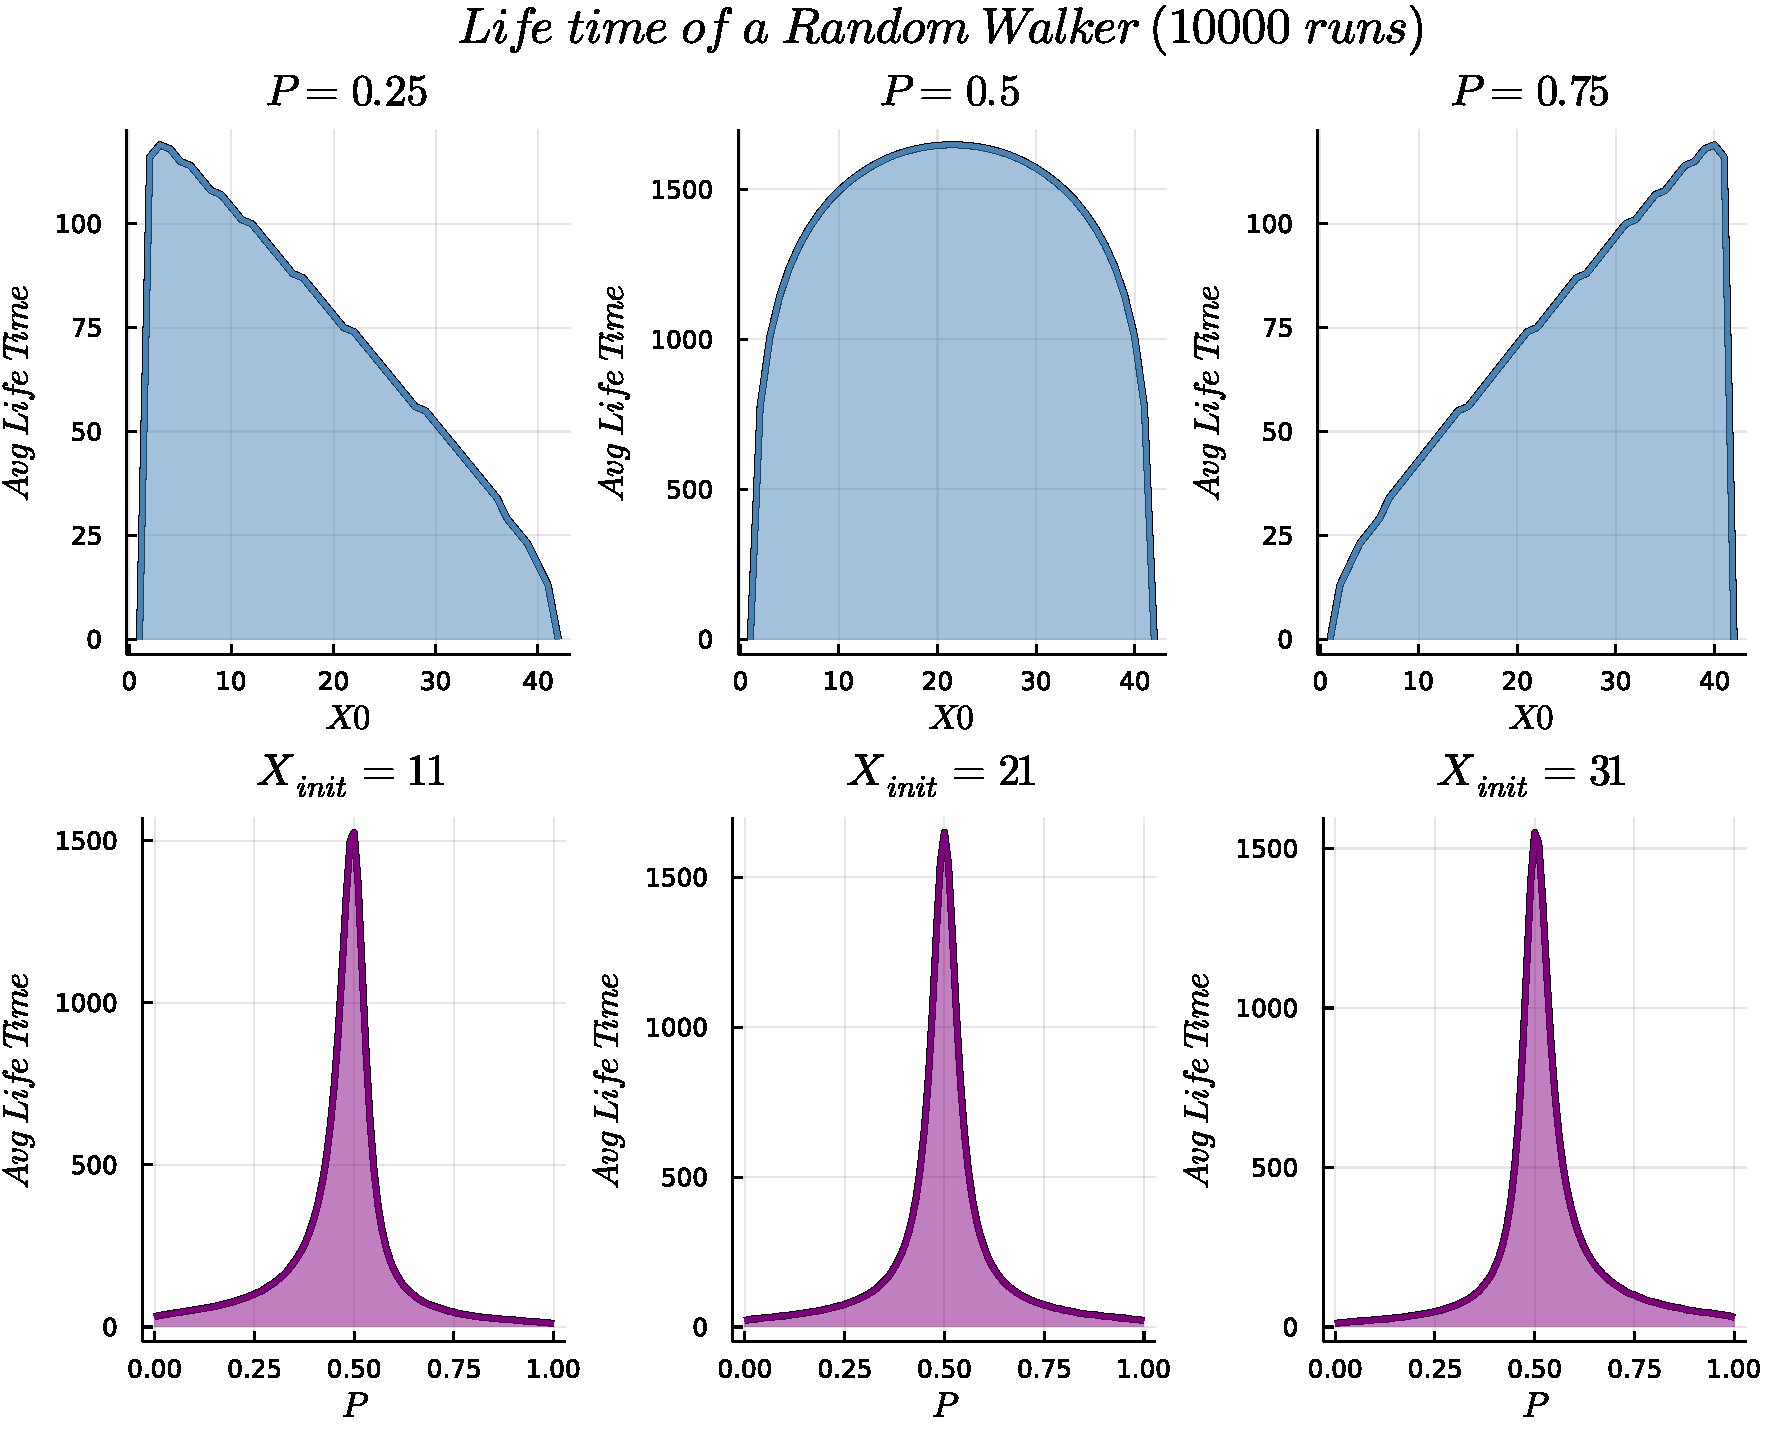
\includegraphics[scale = 0.25]{/Q6/Q6-scat}
        \label{fig:6.1}
        \caption{The plots for several $X_0$ and $P$ and average $X_{final}$ for each.}
    \end{figure}

    \begin{figure}[!htb]
        \centering
        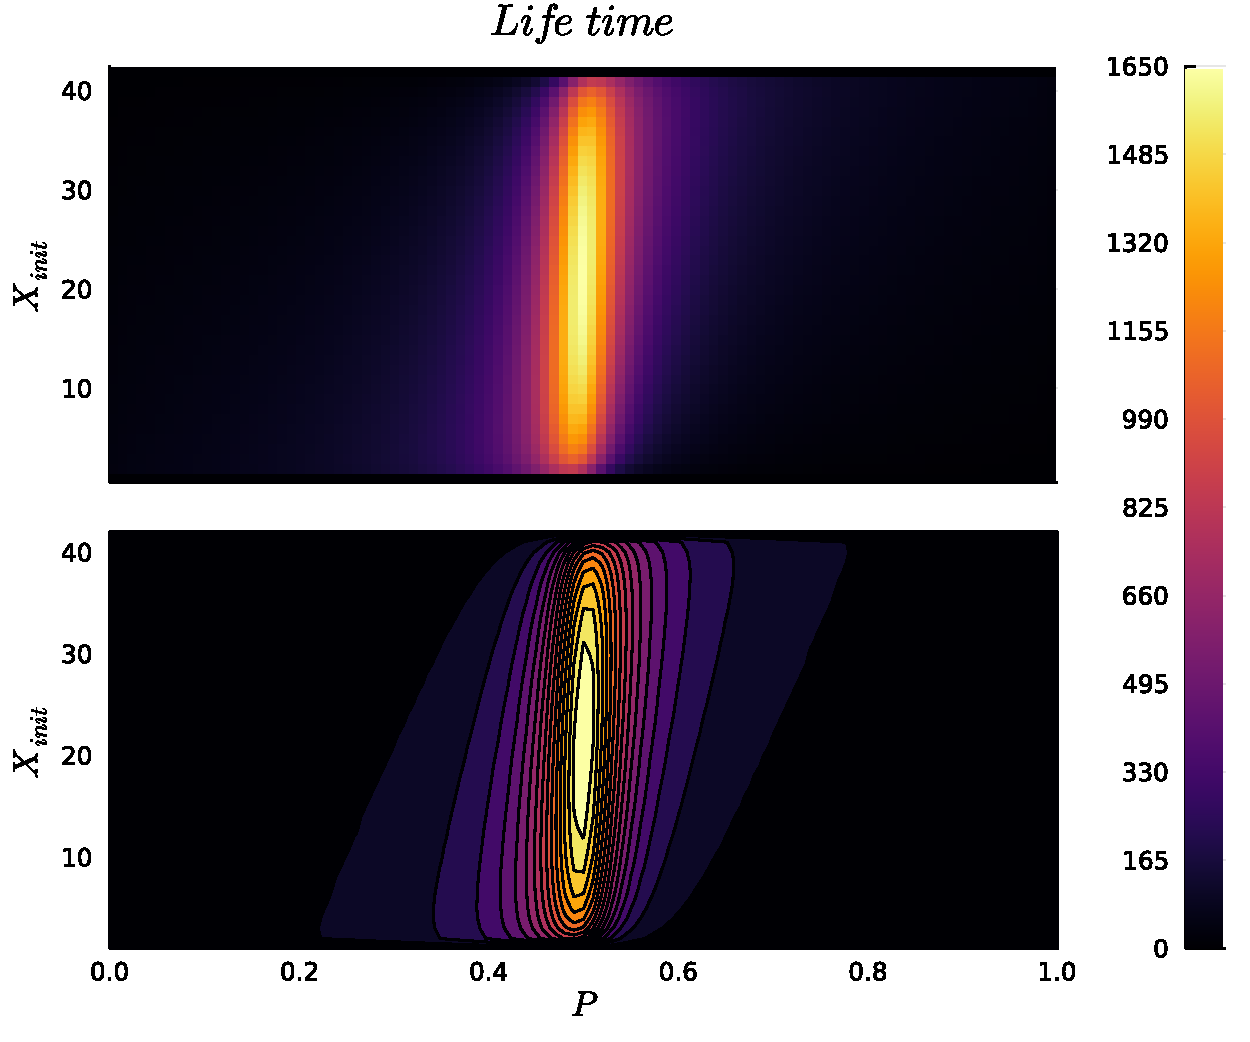
\includegraphics[scale = 0.35]{/Q6/Q6-LT}
        \label{fig:6.2}
        \caption{The contour figures for all possible $X_0$ and $P$ and average $X_{final}$ for each state.}
    \end{figure}

    \centering
    \textbf{The whole data I gathered is in \href{https://github.com/shahmari/ComputationalPhysics-Fall2021/tree/main/ProblemSet4/Data}{this link}}
    
    Thanks for watching :)
\end{document}